
% set document class
\documentclass[10pt]{article}

\usepackage[english]{babel}
\usepackage{underscore}

\usepackage{anyfontsize}

% math packages
\usepackage[utf8]{inputenc}
\usepackage[T1]{fontenc}
\usepackage{geometry} % change paper size
\usepackage{amsmath}
\usepackage{amssymb}
\usepackage{mathtools}
\usepackage{array} 

\usepackage{fontspec}
\setmainfont[Ligatures=TeX,BoldFont={Roboto Medium}]{Roboto Light}
\setmonofont[Ligatures=TeX]{Roboto Mono-Light}

% graphics and tables
\usepackage{graphicx} % add figures
\usepackage[table]{xcolor} % change font color
\usepackage{tikz} % add graphics
\usepackage{multirow} % spanning in tables
\usepackage{caption} % change caption format
\usepackage{booktabs}

\usepackage{setspace} % spacing between paragraphs
\usepackage{url} % allows hyperlinks

% set page margins
\geometry{top = 2in, bottom = 1in, left = 2in, right = 1in}

\usepackage{fancyhdr} % header formating
\pagestyle{fancyplain}
% \rhead{\thepage}
% \fancyhead[R]{\thepage}
\renewcommand{\headrulewidth}{0pt}
%\setlength{\headheight}{15pt} 
\cfoot{}
\rhead{}
\lhead{}

% set paper size
\geometry{letterpaper}

\newcommand\figurenote[1]{\captionsetup{textfont={footnotesize}}\caption*{#1}}

\usepackage{tocloft}
\renewcommand{\cftsecdotsep}{10}
\renewcommand{\cftsecleader}{\cftdotfill{\cftdotsep}}
\renewcommand{\cftsecfont}{{\small\color{black!75}\bfseries}}
\renewcommand{\cftsecpagefont}{{\small\color{black!75}\normalfont}}

% set page numbering
%\pagenumbering{arabic} 
%\pagestyle{plain} % remove page numbering
%\setcounter{page}{1} % remove page number from title page

\usepackage{ragged2e}
\newcolumntype{L}[1]{>{\RaggedRight\arraybackslash}p{#1}}

% adjust spacing
\usepackage{parskip}
% \onehalfspace
\parskip=10pt
\renewcommand{\baselinestretch}{1.5}

%\usepackage[document]{ragged2e}
\hyphenpenalty = 10000
\exhyphenpenalty = 10000

% allow equations to span page breaks
\allowdisplaybreaks

% footnote formatting
\setlength{\footnotesep}{0.5cm}
\usepackage[hang]{footmisc}
\renewcommand{\hangfootparindent}{1em}
\renewcommand{\hangfootparskip}{0pt}
\renewcommand{\footnotemargin}{0.00001pt}
\renewcommand{\footnotelayout}{\hspace{1em}}
\renewcommand\footnoterule{\kern 10pt \hrule width 1in \kern 0pt}

% prevent widow and orphan lines
\widowpenalty10000
\clubpenalty10000

% adjust bullet point style
\renewcommand{\labelitemi}{\raise .3ex\hbox{\footnotesize$\bullet$}}
\renewcommand{\labelitemii}{\raise .3ex\hbox{\footnotesize$\bullet$}}
\renewcommand{\labelitemiii}{\raise .3ex\hbox{\footnotesize$\bullet$}}
\renewcommand{\labelitemiv}{\raise .3ex\hbox{\footnotesize$\bullet$}}

%\usepackage{draftwatermark}
%\SetWatermarkText{\textbf{DRAFT}}
%\SetWatermarkText{\includegraphics{map.png}}
%\SetWatermarkLightness{0.9}
%\SetWatermarkScale{0.9}
%\SetWatermarkColor{black!2}
%\SetWatermarkAngle{0}

%\SetWatermarkHorCenter{}
%\SetWatermarkVerCenter{}

\usepackage{transparent}
\usepackage{eso-pic}

\definecolor{myblue}{HTML}{4A749E}
\definecolor{mypurple}{HTML}{5D1451}

\definecolor{background}{HTML}{EEF6FD}

\usepackage{tcolorbox}
\newtcbox{\codebox}{nobeforeafter,tcbox raise base,colback=black!5,colframe=black!10,coltext=black!75,boxrule=0.5pt,arc=3pt,boxsep=0pt,
left=3pt,right=3pt,top=3pt,bottom=3pt}

\newtcbox{\variablebox}{nobeforeafter,tcbox raise base,colback=mypurple!20,colframe=mypurple!40,coltext=black!75,boxrule=0.5pt,arc=3pt,boxsep=0pt,
left=3pt,right=3pt,top=3pt,bottom=3pt}

\newcommand{\code}[1]{\codebox{{\footnotesize\texttt{#1}}}}

\newcommand{\variable}[1]{\variablebox{{\footnotesize\texttt{#1}}}}

\newcommand{\dataset}[1]{\variablebox{{\footnotesize\texttt{#1}}}}

%\newcommand{\myline}{\vspace{5pt}{\color{gray!40} \rule[3pt]{\textwidth}{0.5pt}}\vspace{5pt}}

\newcommand{\highlight}[1]{{\color{mypurple} \textbf{#1}}}

\newcommand{\myline}{{\color{gray!40} \rule[3pt]{\textwidth}{0.5pt}}}

\newcommand{\separator}{\vspace{20pt}}

\usepackage[colorlinks=true,linkcolor=mypurple,citecolor=mypurple,urlcolor=mypurple,breaklinks=true]{hyperref}

\newcommand\sidebar{
\begin{tikzpicture}[remember picture,overlay, shift={(current page.south west)}]
%\fill[background] (0in, 0in) rectangle ++(1.5in, 9in); % side bar
\draw[line width = 1pt, color = black!10] (5.5in, 11in) -- (5.5in,10in); % header line
\fill[mypurple] (0, 10.75in) rectangle ++ (8.5in, 0.25in); % header bar
\fill[black!10] (0, 0) rectangle ++ (8.5in, 0.5in); % footer bar
\fill[mypurple] (0in, 8in) rectangle ++(0.5in, 1.5in); % page number box
%\fill[black!10] (0.25in, 10in) rectangle ++(2in, 0.5in); % title box
\draw (0.25in, 8.1in) node[anchor = south] {{\color{white}\large\thepage}};
%\draw (5.55in,10in) node[anchor = south west] {{\small \color{black!75} Joshua C. Fjelstul, Ph.D.}};
\draw (5.55in,10.275in) node[anchor = south west] {{\large\color{mypurple}\textbf{United Kingdom Codebook}}};
%\draw (0.25in,0.25in) node[anchor = west] {{\small \color{black!40} Washington University in St.\ Louis \hspace{10pt} | \hspace{10pt} Emory University}};
%\draw (0.3in,10.25in) node[anchor = west] {\color{black!75}\normalsize Judgments Dataset};
\end{tikzpicture}
}

\newcommand\cover{
\begin{tikzpicture}[remember picture,overlay, shift={(current page.south west)}]
\draw (-4.25in,-1in) node[anchor = south west] {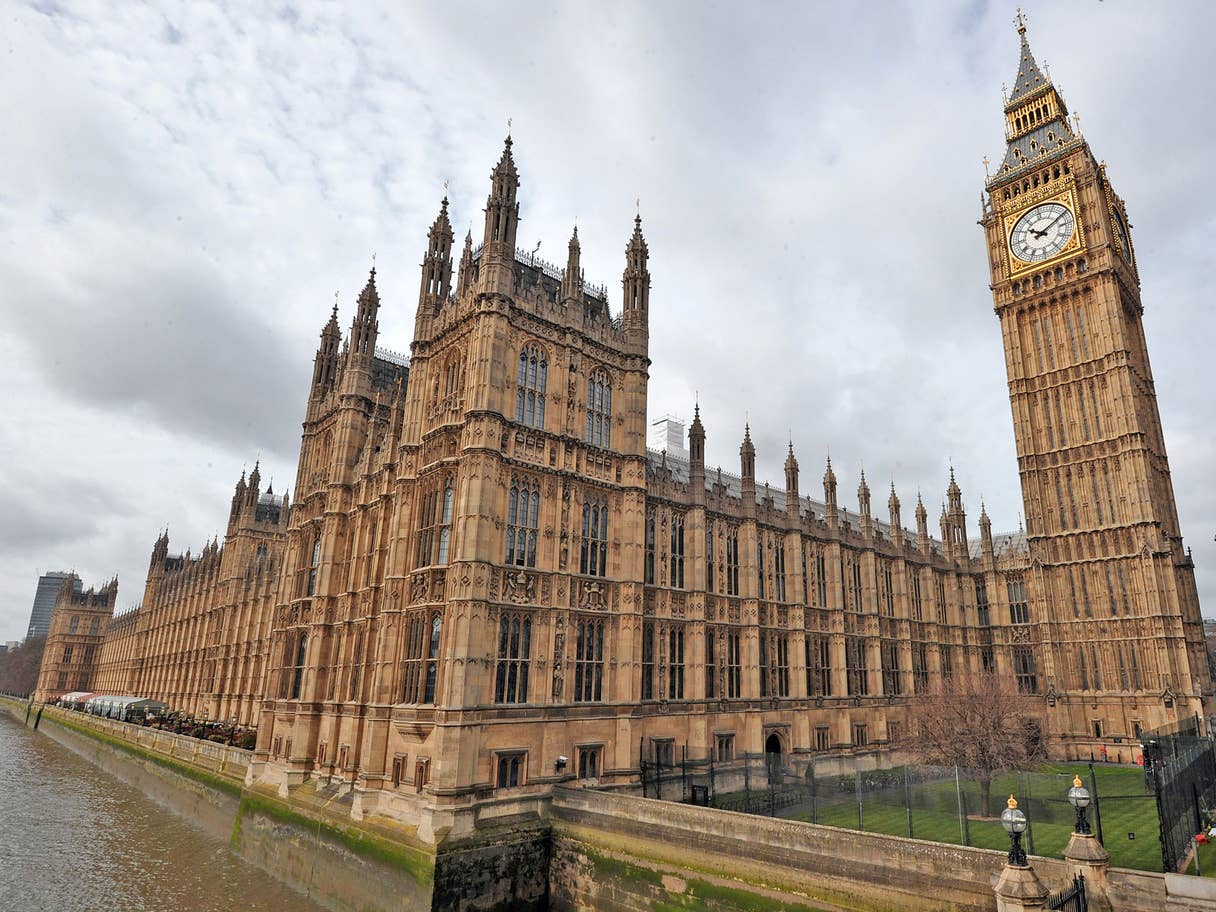
\includegraphics[height=9.7in]{parliament-v2.jpg}};
\fill[mypurple] (0, 8.5in) rectangle ++ (8.5in, 2.5in); % header bar
\fill[mypurple] (0, 0) rectangle ++ (8.5in, 0.5in); % footer bar
\fill[black!10] (0, 8.5in) rectangle ++ (8.5in, -0.1in); % top line
\fill[black!10] (0, 0.5in) rectangle ++ (8.5in, 0.1in); % bottom line
\draw (0.5in,10in) node[anchor = west] {{\color{black!10} \fontsize{55}{55}\selectfont \textbf{UNITED KINGDOM} \fontsize{15}{15}\selectfont v 1.0}};
\draw (0.5in,9.1in) node[anchor = west] {{\color{black!10} \fontsize{15}{15}\selectfont The \textbf{British House of Commons} Codebook}};
%\draw (0.5in,0.25in) node[anchor = west] {{\color{black!10} \fontsize{12}{12}\selectfont Joshua C. Fjelstul, Ph.D.}};
\end{tikzpicture}
}

\newcommand\background{
\begin{tikzpicture}[remember picture,overlay]
  \fill[mypurple] (current page.north west) rectangle ++(\paperwidth,-0.25in);
  \fill[mypurple] (current page.south west) rectangle ++(\paperwidth,0.25in);
\end{tikzpicture}
}

\AddToShipoutPicture{
\sidebar
%\ifnum\value{page}=1{\cover}
}


%\AddToShipoutPictureBG{
%	\AtPageCenter{
%		\put(0, 0)
%			\transparent{0.4}\includegraphics[width=0.8\paperwidth]{map}
%		}
%	}
%}













